\documentclass{book}
\usepackage[a4paper,top=2.5cm,bottom=2.5cm,left=2.5cm,right=2.5cm]{geometry}
\usepackage{makeidx}
\usepackage{natbib}
\usepackage{graphicx}
\usepackage{multicol}
\usepackage{float}
\usepackage{listings}
\usepackage{color}
\usepackage{ifthen}
\usepackage[table]{xcolor}
\usepackage{textcomp}
\usepackage{alltt}
\usepackage{ifpdf}
\ifpdf
\usepackage[pdftex,
            pagebackref=true,
            colorlinks=true,
            linkcolor=blue,
            unicode
           ]{hyperref}
\else
\usepackage[ps2pdf,
            pagebackref=true,
            colorlinks=true,
            linkcolor=blue,
            unicode
           ]{hyperref}
\usepackage{pspicture}
\fi
\usepackage[utf8]{inputenc}
\usepackage{mathptmx}
\usepackage[scaled=.90]{helvet}
\usepackage{courier}
\usepackage{sectsty}
\usepackage{amssymb}
\usepackage[titles]{tocloft}
\usepackage{doxygen}
\lstset{language=C++,inputencoding=utf8,basicstyle=\footnotesize,breaklines=true,breakatwhitespace=true,tabsize=4,numbers=left }
\makeindex
\setcounter{tocdepth}{3}
\renewcommand{\footrulewidth}{0.4pt}
\renewcommand{\familydefault}{\sfdefault}
\hfuzz=15pt
\setlength{\emergencystretch}{15pt}
\hbadness=750
\tolerance=750
\begin{document}
\hypersetup{pageanchor=false,citecolor=blue}
\begin{titlepage}
\vspace*{7cm}
\begin{center}
{\Large Corrupted \\[1ex]\large 1.\-0 }\\
\vspace*{1cm}
{\large Generated by Doxygen 1.8.2}\\
\vspace*{0.5cm}
{\small Thu Oct 11 2012 15:08:37}\\
\end{center}
\end{titlepage}
\clearemptydoublepage
\pagenumbering{roman}
\tableofcontents
\clearemptydoublepage
\pagenumbering{arabic}
\hypersetup{pageanchor=true,citecolor=blue}
\chapter{Hierarchical Index}
\section{Class Hierarchy}
This inheritance list is sorted roughly, but not completely, alphabetically\-:\begin{DoxyCompactList}
\item \contentsline{section}{Actor}{\pageref{class_actor}}{}
\begin{DoxyCompactList}
\item \contentsline{section}{Character}{\pageref{class_character}}{}
\begin{DoxyCompactList}
\item \contentsline{section}{Player}{\pageref{class_player}}{}
\end{DoxyCompactList}
\end{DoxyCompactList}
\item \contentsline{section}{Game}{\pageref{class_game}}{}
\item \contentsline{section}{Vector2f}{\pageref{class_vector2f}}{}
\end{DoxyCompactList}

\chapter{Class Index}
\section{Class List}
Here are the classes, structs, unions and interfaces with brief descriptions\-:\begin{DoxyCompactList}
\item\contentsline{section}{\hyperlink{class_actor}{Actor} }{\pageref{class_actor}}{}
\item\contentsline{section}{\hyperlink{class_character}{Character} }{\pageref{class_character}}{}
\item\contentsline{section}{\hyperlink{class_game}{Game} }{\pageref{class_game}}{}
\item\contentsline{section}{\hyperlink{class_player}{Player} }{\pageref{class_player}}{}
\item\contentsline{section}{\hyperlink{class_vector2f}{Vector2f} }{\pageref{class_vector2f}}{}
\end{DoxyCompactList}

\chapter{File Index}
\section{File List}
Here is a list of all files with brief descriptions\-:\begin{DoxyCompactList}
\item\contentsline{section}{Game\-Project/\-Game\-Project/\hyperlink{_actor_8cpp}{Actor.\-cpp} }{\pageref{_actor_8cpp}}{}
\item\contentsline{section}{Game\-Project/\-Game\-Project/\hyperlink{_actor_8h}{Actor.\-h} }{\pageref{_actor_8h}}{}
\item\contentsline{section}{Game\-Project/\-Game\-Project/\hyperlink{_character_8cpp}{Character.\-cpp} }{\pageref{_character_8cpp}}{}
\item\contentsline{section}{Game\-Project/\-Game\-Project/\hyperlink{_character_8h}{Character.\-h} }{\pageref{_character_8h}}{}
\item\contentsline{section}{Game\-Project/\-Game\-Project/\hyperlink{_enemy_8h}{Enemy.\-h} }{\pageref{_enemy_8h}}{}
\item\contentsline{section}{Game\-Project/\-Game\-Project/\hyperlink{_enemy_factory_8h}{Enemy\-Factory.\-h} }{\pageref{_enemy_factory_8h}}{}
\item\contentsline{section}{Game\-Project/\-Game\-Project/\hyperlink{_enemy_handler_8h}{Enemy\-Handler.\-h} }{\pageref{_enemy_handler_8h}}{}
\item\contentsline{section}{Game\-Project/\-Game\-Project/\hyperlink{_environment_8h}{Environment.\-h} }{\pageref{_environment_8h}}{}
\item\contentsline{section}{Game\-Project/\-Game\-Project/\hyperlink{_game_8cpp}{Game.\-cpp} }{\pageref{_game_8cpp}}{}
\item\contentsline{section}{Game\-Project/\-Game\-Project/\hyperlink{_game_8h}{Game.\-h} }{\pageref{_game_8h}}{}
\item\contentsline{section}{Game\-Project/\-Game\-Project/\hyperlink{main_8cpp}{main.\-cpp} }{\pageref{main_8cpp}}{}
\item\contentsline{section}{Game\-Project/\-Game\-Project/\hyperlink{_objects_8h}{Objects.\-h} }{\pageref{_objects_8h}}{}
\item\contentsline{section}{Game\-Project/\-Game\-Project/\hyperlink{_player_8cpp}{Player.\-cpp} }{\pageref{_player_8cpp}}{}
\item\contentsline{section}{Game\-Project/\-Game\-Project/\hyperlink{_player_8h}{Player.\-h} }{\pageref{_player_8h}}{}
\item\contentsline{section}{Game\-Project/\-Game\-Project/\hyperlink{_scene_handler_8h}{Scene\-Handler.\-h} }{\pageref{_scene_handler_8h}}{}
\item\contentsline{section}{Game\-Project/\-Game\-Project/\hyperlink{_vector2f_8cpp}{Vector2f.\-cpp} }{\pageref{_vector2f_8cpp}}{}
\item\contentsline{section}{Game\-Project/\-Game\-Project/\hyperlink{_vector2f_8h}{Vector2f.\-h} }{\pageref{_vector2f_8h}}{}
\end{DoxyCompactList}

\chapter{Class Documentation}
\hypertarget{class_actor}{\section{Actor Class Reference}
\label{class_actor}\index{Actor@{Actor}}
}


{\ttfamily \#include $<$Actor.\-h$>$}

Inheritance diagram for Actor\-:\begin{figure}[H]
\begin{center}
\leavevmode
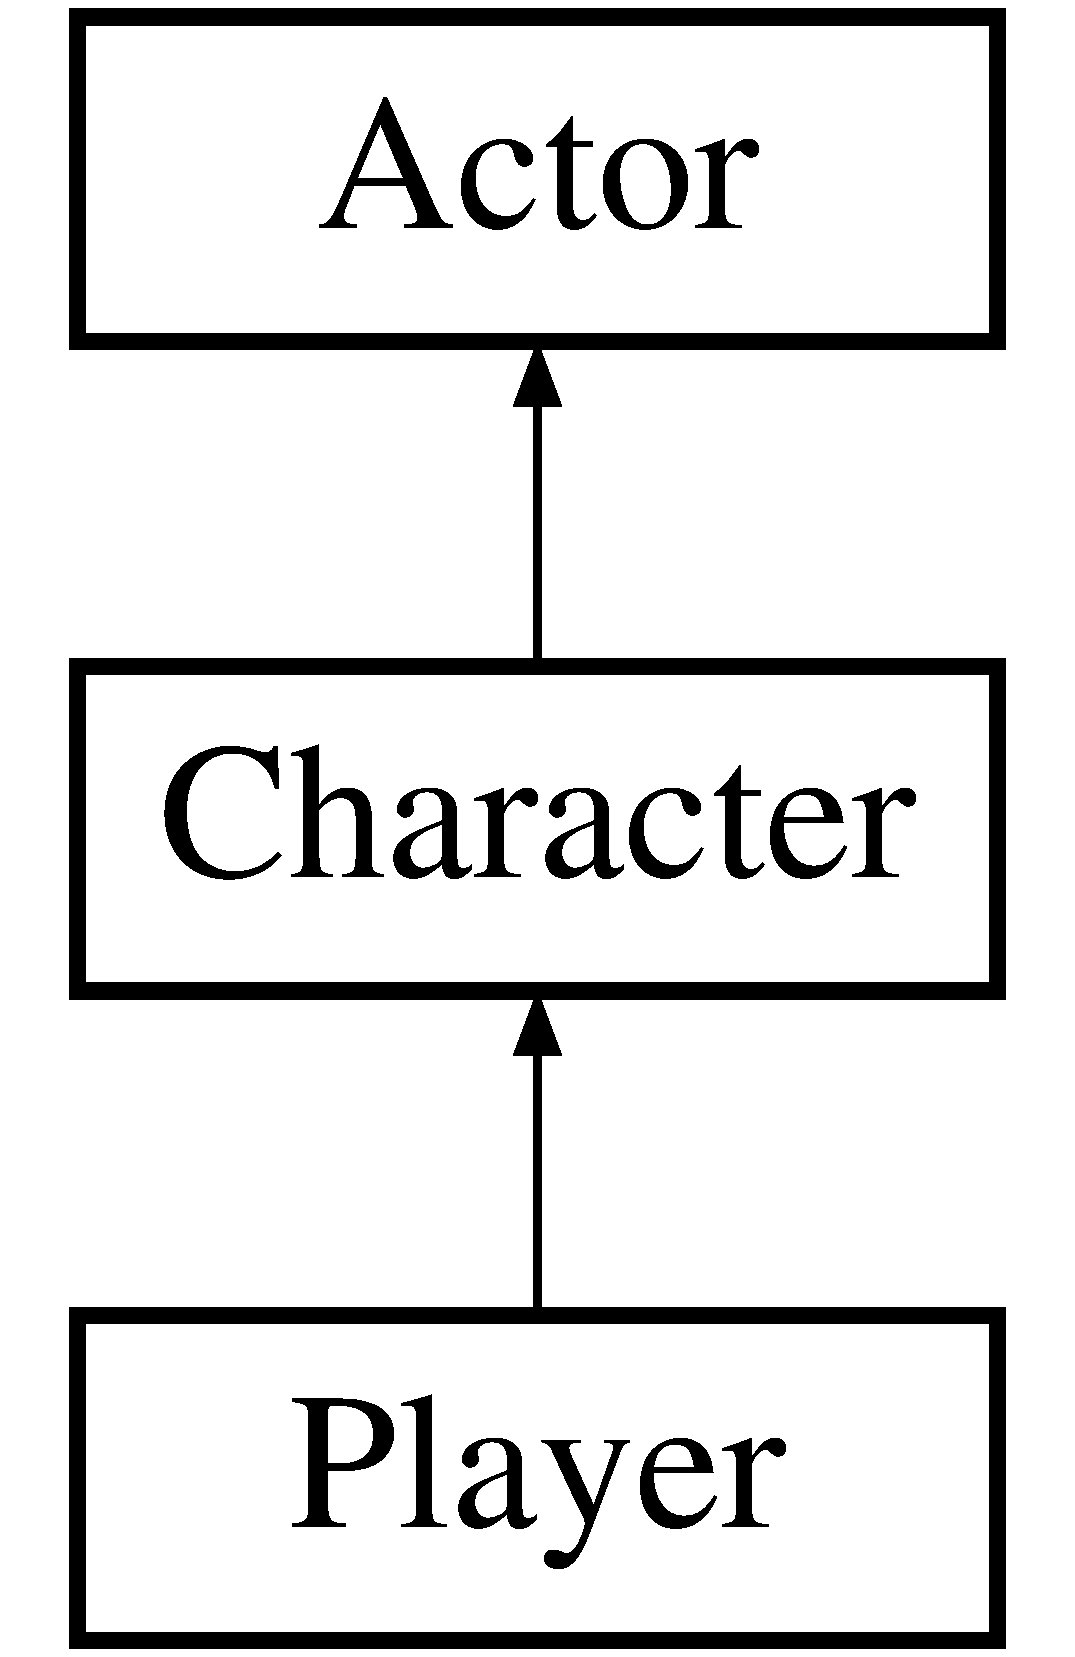
\includegraphics[height=3.000000cm]{class_actor}
\end{center}
\end{figure}
\subsection*{Public Member Functions}
\begin{DoxyCompactItemize}
\item 
bool \hyperlink{class_actor_a60c7df9b26c488c69cc6c3ade1d5e405}{load\-Content} ()
\item 
void \hyperlink{class_actor_ac8bc898122ba0aaa8383187525edeaf6}{draw} ()
\item 
\hyperlink{class_actor_a2a0ff4335a1ee9096df90f288c026c8b}{Actor} ()
\item 
\hyperlink{class_actor_ab8cede14b717ebbdb29f8164178c876a}{Actor} (int x, int y)
\item 
\hyperlink{class_actor_a6be1c55f99c17cd3ed53c98c26222b0e}{Actor} (int x, int y, sf\-::\-Sprite sprite)
\item 
\hyperlink{class_actor_a55bb8f581a59fe3d2be4a90c29ce1e7a}{Actor} (sf\-::\-Sprite sprite)
\end{DoxyCompactItemize}
\subsection*{Protected Member Functions}
\begin{DoxyCompactItemize}
\item 
void \hyperlink{class_actor_a04ab5a0b1f9d0528a45696befcb97e1f}{set\-Position} (int x, int y)
\item 
\hyperlink{class_vector2f}{Vector2f} $\ast$ \hyperlink{class_actor_a9ec6f26161cadc978f8ba6d2c5ba1377}{get\-Position} ()
\item 
void \hyperlink{class_actor_a59bd7eda50ba530619a95c1758b8069b}{set\-Sprite} ()
\end{DoxyCompactItemize}
\subsection*{Private Attributes}
\begin{DoxyCompactItemize}
\item 
sf\-::\-Texture \hyperlink{class_actor_a6cb7c1cd422797dc023776229b69eb6f}{m\-\_\-\-Texture}
\item 
\hyperlink{class_vector2f}{Vector2f} \hyperlink{class_actor_a7c6e321fb5b42e47c98ad548f2ef4122}{m\-\_\-\-Position}
\item 
sf\-::\-Sprite \hyperlink{class_actor_a043c786e0933f1cfdaded0d5e1d504e6}{m\-\_\-\-Sprite}
\end{DoxyCompactItemize}


\subsection{Constructor \& Destructor Documentation}
\hypertarget{class_actor_a2a0ff4335a1ee9096df90f288c026c8b}{\index{Actor@{Actor}!Actor@{Actor}}
\index{Actor@{Actor}!Actor@{Actor}}
\subsubsection[{Actor}]{\setlength{\rightskip}{0pt plus 5cm}Actor\-::\-Actor (
\begin{DoxyParamCaption}
{}
\end{DoxyParamCaption}
)}}\label{class_actor_a2a0ff4335a1ee9096df90f288c026c8b}
\hypertarget{class_actor_ab8cede14b717ebbdb29f8164178c876a}{\index{Actor@{Actor}!Actor@{Actor}}
\index{Actor@{Actor}!Actor@{Actor}}
\subsubsection[{Actor}]{\setlength{\rightskip}{0pt plus 5cm}Actor\-::\-Actor (
\begin{DoxyParamCaption}
\item[{int}]{x, }
\item[{int}]{y}
\end{DoxyParamCaption}
)}}\label{class_actor_ab8cede14b717ebbdb29f8164178c876a}
\hypertarget{class_actor_a6be1c55f99c17cd3ed53c98c26222b0e}{\index{Actor@{Actor}!Actor@{Actor}}
\index{Actor@{Actor}!Actor@{Actor}}
\subsubsection[{Actor}]{\setlength{\rightskip}{0pt plus 5cm}Actor\-::\-Actor (
\begin{DoxyParamCaption}
\item[{int}]{x, }
\item[{int}]{y, }
\item[{sf\-::\-Sprite}]{sprite}
\end{DoxyParamCaption}
)}}\label{class_actor_a6be1c55f99c17cd3ed53c98c26222b0e}
\hypertarget{class_actor_a55bb8f581a59fe3d2be4a90c29ce1e7a}{\index{Actor@{Actor}!Actor@{Actor}}
\index{Actor@{Actor}!Actor@{Actor}}
\subsubsection[{Actor}]{\setlength{\rightskip}{0pt plus 5cm}Actor\-::\-Actor (
\begin{DoxyParamCaption}
\item[{sf\-::\-Sprite}]{sprite}
\end{DoxyParamCaption}
)}}\label{class_actor_a55bb8f581a59fe3d2be4a90c29ce1e7a}


\subsection{Member Function Documentation}
\hypertarget{class_actor_ac8bc898122ba0aaa8383187525edeaf6}{\index{Actor@{Actor}!draw@{draw}}
\index{draw@{draw}!Actor@{Actor}}
\subsubsection[{draw}]{\setlength{\rightskip}{0pt plus 5cm}void Actor\-::draw (
\begin{DoxyParamCaption}
{}
\end{DoxyParamCaption}
)}}\label{class_actor_ac8bc898122ba0aaa8383187525edeaf6}
\hypertarget{class_actor_a9ec6f26161cadc978f8ba6d2c5ba1377}{\index{Actor@{Actor}!get\-Position@{get\-Position}}
\index{get\-Position@{get\-Position}!Actor@{Actor}}
\subsubsection[{get\-Position}]{\setlength{\rightskip}{0pt plus 5cm}{\bf Vector2f} $\ast$ Actor\-::get\-Position (
\begin{DoxyParamCaption}
{}
\end{DoxyParamCaption}
)\hspace{0.3cm}{\ttfamily [protected]}}}\label{class_actor_a9ec6f26161cadc978f8ba6d2c5ba1377}
\hypertarget{class_actor_a60c7df9b26c488c69cc6c3ade1d5e405}{\index{Actor@{Actor}!load\-Content@{load\-Content}}
\index{load\-Content@{load\-Content}!Actor@{Actor}}
\subsubsection[{load\-Content}]{\setlength{\rightskip}{0pt plus 5cm}bool Actor\-::load\-Content (
\begin{DoxyParamCaption}
{}
\end{DoxyParamCaption}
)}}\label{class_actor_a60c7df9b26c488c69cc6c3ade1d5e405}
\hypertarget{class_actor_a04ab5a0b1f9d0528a45696befcb97e1f}{\index{Actor@{Actor}!set\-Position@{set\-Position}}
\index{set\-Position@{set\-Position}!Actor@{Actor}}
\subsubsection[{set\-Position}]{\setlength{\rightskip}{0pt plus 5cm}void Actor\-::set\-Position (
\begin{DoxyParamCaption}
\item[{int}]{x, }
\item[{int}]{y}
\end{DoxyParamCaption}
)\hspace{0.3cm}{\ttfamily [protected]}}}\label{class_actor_a04ab5a0b1f9d0528a45696befcb97e1f}
\hypertarget{class_actor_a59bd7eda50ba530619a95c1758b8069b}{\index{Actor@{Actor}!set\-Sprite@{set\-Sprite}}
\index{set\-Sprite@{set\-Sprite}!Actor@{Actor}}
\subsubsection[{set\-Sprite}]{\setlength{\rightskip}{0pt plus 5cm}void Actor\-::set\-Sprite (
\begin{DoxyParamCaption}
{}
\end{DoxyParamCaption}
)\hspace{0.3cm}{\ttfamily [protected]}}}\label{class_actor_a59bd7eda50ba530619a95c1758b8069b}


\subsection{Member Data Documentation}
\hypertarget{class_actor_a7c6e321fb5b42e47c98ad548f2ef4122}{\index{Actor@{Actor}!m\-\_\-\-Position@{m\-\_\-\-Position}}
\index{m\-\_\-\-Position@{m\-\_\-\-Position}!Actor@{Actor}}
\subsubsection[{m\-\_\-\-Position}]{\setlength{\rightskip}{0pt plus 5cm}{\bf Vector2f} Actor\-::m\-\_\-\-Position\hspace{0.3cm}{\ttfamily [private]}}}\label{class_actor_a7c6e321fb5b42e47c98ad548f2ef4122}
\hypertarget{class_actor_a043c786e0933f1cfdaded0d5e1d504e6}{\index{Actor@{Actor}!m\-\_\-\-Sprite@{m\-\_\-\-Sprite}}
\index{m\-\_\-\-Sprite@{m\-\_\-\-Sprite}!Actor@{Actor}}
\subsubsection[{m\-\_\-\-Sprite}]{\setlength{\rightskip}{0pt plus 5cm}sf\-::\-Sprite Actor\-::m\-\_\-\-Sprite\hspace{0.3cm}{\ttfamily [private]}}}\label{class_actor_a043c786e0933f1cfdaded0d5e1d504e6}
\hypertarget{class_actor_a6cb7c1cd422797dc023776229b69eb6f}{\index{Actor@{Actor}!m\-\_\-\-Texture@{m\-\_\-\-Texture}}
\index{m\-\_\-\-Texture@{m\-\_\-\-Texture}!Actor@{Actor}}
\subsubsection[{m\-\_\-\-Texture}]{\setlength{\rightskip}{0pt plus 5cm}sf\-::\-Texture Actor\-::m\-\_\-\-Texture\hspace{0.3cm}{\ttfamily [private]}}}\label{class_actor_a6cb7c1cd422797dc023776229b69eb6f}


The documentation for this class was generated from the following files\-:\begin{DoxyCompactItemize}
\item 
Game\-Project/\-Game\-Project/\hyperlink{_actor_8h}{Actor.\-h}\item 
Game\-Project/\-Game\-Project/\hyperlink{_actor_8cpp}{Actor.\-cpp}\end{DoxyCompactItemize}

\hypertarget{class_character}{\section{Character Class Reference}
\label{class_character}\index{Character@{Character}}
}


{\ttfamily \#include $<$Character.\-h$>$}

Inheritance diagram for Character\-:\begin{figure}[H]
\begin{center}
\leavevmode
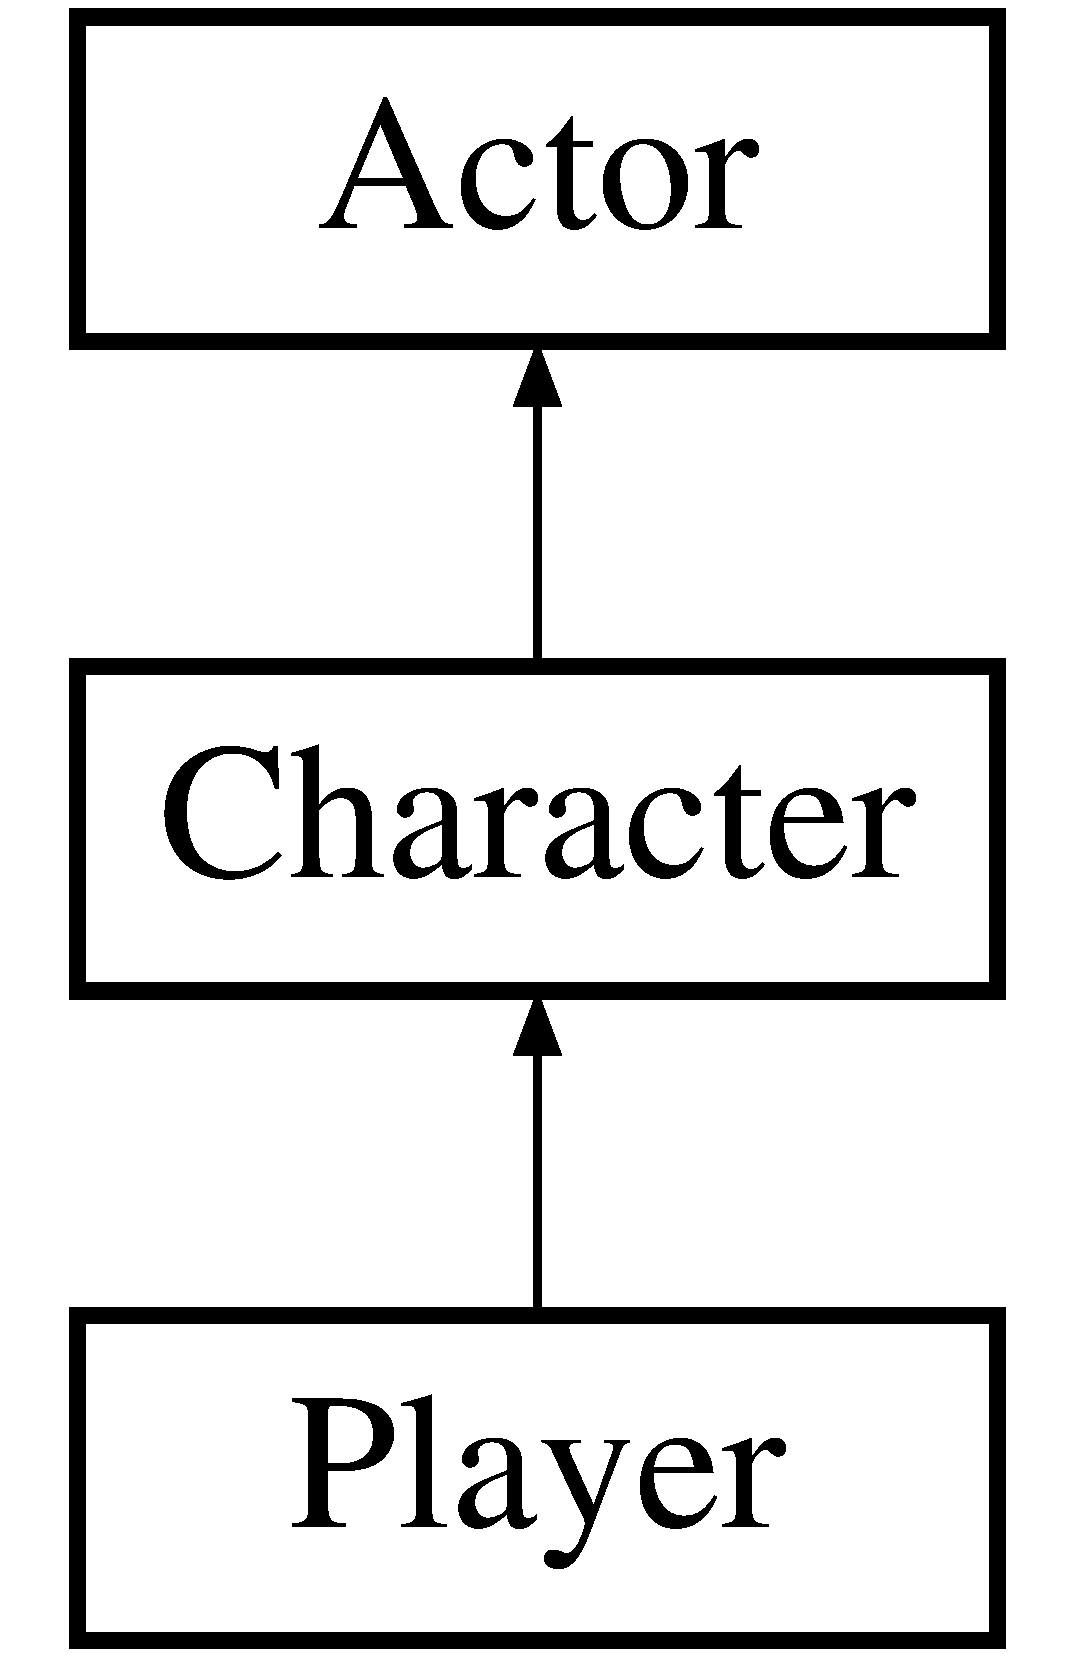
\includegraphics[height=3.000000cm]{class_character}
\end{center}
\end{figure}
\subsection*{Public Member Functions}
\begin{DoxyCompactItemize}
\item 
void \hyperlink{class_character_a891042a5f9ba38a4ab98d79e32a590b9}{attack} ()
\item 
short \hyperlink{class_character_a71e26e0edbb4182414827b997bea7be2}{get\-Health} ()
\item 
short \hyperlink{class_character_a6f53d06b8eb41bebb45750676a2f2b3d}{get\-Damage} ()
\item 
short \hyperlink{class_character_a50c26b239e9687ba5b34665a65a11dbe}{get\-Speed} ()
\item 
short \hyperlink{class_character_ad607ba44fdccc8b571f19194cc205dd4}{get\-Toughness} ()
\item 
short \hyperlink{class_character_a79a7ef5e8b1bdca05424fe611fe056b9}{get\-Intelligence} ()
\item 
short \hyperlink{class_character_a56dc21cdc1c460fac9ab013e09a36dd9}{get\-Strength} ()
\item 
short \hyperlink{class_character_a621cb6b6e50c35ce431b914dd300b16b}{get\-Level} ()
\item 
bool $\ast$ \hyperlink{class_character_a00d426ba5c22e935add036831a100bc8}{get\-Abilities} ()
\item 
void \hyperlink{class_character_ade340e0ec4e25b8f86615323f588eb9c}{move\-Horizontal} (bool horizontal\-Movement)
\item 
void \hyperlink{class_character_a9f46f32c23ef47d0454fc6bb00b95294}{move\-Vertical} (bool vertical\-Movement)
\item 
void \hyperlink{class_character_ae6b11b3e6a84287216630ecc355ab8e3}{show\-Damage} ()
\item 
void \hyperlink{class_character_a84a7de8166aa93320511fc4fc4e77b44}{show\-Health} ()
\end{DoxyCompactItemize}
\subsection*{Protected Member Functions}
\begin{DoxyCompactItemize}
\item 
\hyperlink{class_character_adc27bdd255876169bad2ed0bae0cffb5}{Character} ()
\item 
\hyperlink{class_character_a08203d27a9066d6e658eb78940b5bb06}{Character} (int variables\-Here)
\end{DoxyCompactItemize}
\subsection*{Private Types}
\begin{DoxyCompactItemize}
\item 
enum \hyperlink{class_character_ab6fbd7c75b53c7bcd4701cafb8715ba1}{abilities} \{ \hyperlink{class_character_ab6fbd7c75b53c7bcd4701cafb8715ba1aa244fdde78c2cb6d1db99a93597d2492}{F\-I\-R\-E\-B\-A\-L\-L}, 
\hyperlink{class_character_ab6fbd7c75b53c7bcd4701cafb8715ba1aa6de6b6a3e7651a31fde58c82b6baaa2}{F\-R\-O\-S\-T\-B\-O\-L\-T}, 
\hyperlink{class_character_ab6fbd7c75b53c7bcd4701cafb8715ba1a194cb46b225b19308b6859bebb69e265}{L\-I\-G\-H\-T\-N\-I\-N\-G\-B\-O\-L\-T}
 \}
\end{DoxyCompactItemize}
\subsection*{Private Attributes}
\begin{DoxyCompactItemize}
\item 
\hyperlink{class_character_ab6fbd7c75b53c7bcd4701cafb8715ba1}{abilities} \hyperlink{class_character_a8ce5038804317cc41b3672b2f77aee77}{m\-\_\-e\-Abilities}
\item 
short \hyperlink{class_character_a50138cd901b1f729a01e5e018bf63256}{m\-\_\-sh\-Health}
\item 
short \hyperlink{class_character_a504b1237f1321ae15abe0f359295a0d7}{m\-\_\-sh\-Damage}
\item 
short \hyperlink{class_character_abb0c7e556292b3d93d52e9c9f9db6258}{m\-\_\-sh\-Speed}
\item 
short \hyperlink{class_character_adaaccd5040167071f5aa3281cade4c19}{m\-\_\-sh\-Toughness}
\item 
short \hyperlink{class_character_a2319f838d38029537e1e5c6e24c24ebb}{m\-\_\-sh\-Intelligence}
\item 
short \hyperlink{class_character_a500cced8623c4cca096e0555795b6025}{m\-\_\-sh\-Strength}
\item 
short \hyperlink{class_character_afd011d8f32a2f60e3ef604a191d3ebf4}{m\-\_\-sh\-Level}
\item 
bool $\ast$ \hyperlink{class_character_a9251eb7762d3ae204f3034bfb5e83476}{m\-\_\-b\-Abilities}
\end{DoxyCompactItemize}


\subsection{Member Enumeration Documentation}
\hypertarget{class_character_ab6fbd7c75b53c7bcd4701cafb8715ba1}{\index{Character@{Character}!abilities@{abilities}}
\index{abilities@{abilities}!Character@{Character}}
\subsubsection[{abilities}]{\setlength{\rightskip}{0pt plus 5cm}enum {\bf Character\-::abilities}\hspace{0.3cm}{\ttfamily [private]}}}\label{class_character_ab6fbd7c75b53c7bcd4701cafb8715ba1}
\begin{Desc}
\item[Enumerator\-: ]\par
\begin{description}
\index{F\-I\-R\-E\-B\-A\-L\-L@{F\-I\-R\-E\-B\-A\-L\-L}!Character@{Character}}\index{Character@{Character}!F\-I\-R\-E\-B\-A\-L\-L@{F\-I\-R\-E\-B\-A\-L\-L}}\item[{\em 
\hypertarget{class_character_ab6fbd7c75b53c7bcd4701cafb8715ba1aa244fdde78c2cb6d1db99a93597d2492}{F\-I\-R\-E\-B\-A\-L\-L}\label{class_character_ab6fbd7c75b53c7bcd4701cafb8715ba1aa244fdde78c2cb6d1db99a93597d2492}
}]\index{F\-R\-O\-S\-T\-B\-O\-L\-T@{F\-R\-O\-S\-T\-B\-O\-L\-T}!Character@{Character}}\index{Character@{Character}!F\-R\-O\-S\-T\-B\-O\-L\-T@{F\-R\-O\-S\-T\-B\-O\-L\-T}}\item[{\em 
\hypertarget{class_character_ab6fbd7c75b53c7bcd4701cafb8715ba1aa6de6b6a3e7651a31fde58c82b6baaa2}{F\-R\-O\-S\-T\-B\-O\-L\-T}\label{class_character_ab6fbd7c75b53c7bcd4701cafb8715ba1aa6de6b6a3e7651a31fde58c82b6baaa2}
}]\index{L\-I\-G\-H\-T\-N\-I\-N\-G\-B\-O\-L\-T@{L\-I\-G\-H\-T\-N\-I\-N\-G\-B\-O\-L\-T}!Character@{Character}}\index{Character@{Character}!L\-I\-G\-H\-T\-N\-I\-N\-G\-B\-O\-L\-T@{L\-I\-G\-H\-T\-N\-I\-N\-G\-B\-O\-L\-T}}\item[{\em 
\hypertarget{class_character_ab6fbd7c75b53c7bcd4701cafb8715ba1a194cb46b225b19308b6859bebb69e265}{L\-I\-G\-H\-T\-N\-I\-N\-G\-B\-O\-L\-T}\label{class_character_ab6fbd7c75b53c7bcd4701cafb8715ba1a194cb46b225b19308b6859bebb69e265}
}]\end{description}
\end{Desc}



\subsection{Constructor \& Destructor Documentation}
\hypertarget{class_character_adc27bdd255876169bad2ed0bae0cffb5}{\index{Character@{Character}!Character@{Character}}
\index{Character@{Character}!Character@{Character}}
\subsubsection[{Character}]{\setlength{\rightskip}{0pt plus 5cm}Character\-::\-Character (
\begin{DoxyParamCaption}
{}
\end{DoxyParamCaption}
)\hspace{0.3cm}{\ttfamily [protected]}}}\label{class_character_adc27bdd255876169bad2ed0bae0cffb5}
\hypertarget{class_character_a08203d27a9066d6e658eb78940b5bb06}{\index{Character@{Character}!Character@{Character}}
\index{Character@{Character}!Character@{Character}}
\subsubsection[{Character}]{\setlength{\rightskip}{0pt plus 5cm}Character\-::\-Character (
\begin{DoxyParamCaption}
\item[{int}]{variables\-Here}
\end{DoxyParamCaption}
)\hspace{0.3cm}{\ttfamily [protected]}}}\label{class_character_a08203d27a9066d6e658eb78940b5bb06}


\subsection{Member Function Documentation}
\hypertarget{class_character_a891042a5f9ba38a4ab98d79e32a590b9}{\index{Character@{Character}!attack@{attack}}
\index{attack@{attack}!Character@{Character}}
\subsubsection[{attack}]{\setlength{\rightskip}{0pt plus 5cm}void Character\-::attack (
\begin{DoxyParamCaption}
{}
\end{DoxyParamCaption}
)}}\label{class_character_a891042a5f9ba38a4ab98d79e32a590b9}
\hypertarget{class_character_a00d426ba5c22e935add036831a100bc8}{\index{Character@{Character}!get\-Abilities@{get\-Abilities}}
\index{get\-Abilities@{get\-Abilities}!Character@{Character}}
\subsubsection[{get\-Abilities}]{\setlength{\rightskip}{0pt plus 5cm}bool $\ast$ Character\-::get\-Abilities (
\begin{DoxyParamCaption}
{}
\end{DoxyParamCaption}
)}}\label{class_character_a00d426ba5c22e935add036831a100bc8}
\hypertarget{class_character_a6f53d06b8eb41bebb45750676a2f2b3d}{\index{Character@{Character}!get\-Damage@{get\-Damage}}
\index{get\-Damage@{get\-Damage}!Character@{Character}}
\subsubsection[{get\-Damage}]{\setlength{\rightskip}{0pt plus 5cm}short Character\-::get\-Damage (
\begin{DoxyParamCaption}
{}
\end{DoxyParamCaption}
)}}\label{class_character_a6f53d06b8eb41bebb45750676a2f2b3d}
\hypertarget{class_character_a71e26e0edbb4182414827b997bea7be2}{\index{Character@{Character}!get\-Health@{get\-Health}}
\index{get\-Health@{get\-Health}!Character@{Character}}
\subsubsection[{get\-Health}]{\setlength{\rightskip}{0pt plus 5cm}short Character\-::get\-Health (
\begin{DoxyParamCaption}
{}
\end{DoxyParamCaption}
)}}\label{class_character_a71e26e0edbb4182414827b997bea7be2}
\hypertarget{class_character_a79a7ef5e8b1bdca05424fe611fe056b9}{\index{Character@{Character}!get\-Intelligence@{get\-Intelligence}}
\index{get\-Intelligence@{get\-Intelligence}!Character@{Character}}
\subsubsection[{get\-Intelligence}]{\setlength{\rightskip}{0pt plus 5cm}short Character\-::get\-Intelligence (
\begin{DoxyParamCaption}
{}
\end{DoxyParamCaption}
)}}\label{class_character_a79a7ef5e8b1bdca05424fe611fe056b9}
\hypertarget{class_character_a621cb6b6e50c35ce431b914dd300b16b}{\index{Character@{Character}!get\-Level@{get\-Level}}
\index{get\-Level@{get\-Level}!Character@{Character}}
\subsubsection[{get\-Level}]{\setlength{\rightskip}{0pt plus 5cm}short Character\-::get\-Level (
\begin{DoxyParamCaption}
{}
\end{DoxyParamCaption}
)}}\label{class_character_a621cb6b6e50c35ce431b914dd300b16b}
\hypertarget{class_character_a50c26b239e9687ba5b34665a65a11dbe}{\index{Character@{Character}!get\-Speed@{get\-Speed}}
\index{get\-Speed@{get\-Speed}!Character@{Character}}
\subsubsection[{get\-Speed}]{\setlength{\rightskip}{0pt plus 5cm}short Character\-::get\-Speed (
\begin{DoxyParamCaption}
{}
\end{DoxyParamCaption}
)}}\label{class_character_a50c26b239e9687ba5b34665a65a11dbe}
\hypertarget{class_character_a56dc21cdc1c460fac9ab013e09a36dd9}{\index{Character@{Character}!get\-Strength@{get\-Strength}}
\index{get\-Strength@{get\-Strength}!Character@{Character}}
\subsubsection[{get\-Strength}]{\setlength{\rightskip}{0pt plus 5cm}short Character\-::get\-Strength (
\begin{DoxyParamCaption}
{}
\end{DoxyParamCaption}
)}}\label{class_character_a56dc21cdc1c460fac9ab013e09a36dd9}
\hypertarget{class_character_ad607ba44fdccc8b571f19194cc205dd4}{\index{Character@{Character}!get\-Toughness@{get\-Toughness}}
\index{get\-Toughness@{get\-Toughness}!Character@{Character}}
\subsubsection[{get\-Toughness}]{\setlength{\rightskip}{0pt plus 5cm}short Character\-::get\-Toughness (
\begin{DoxyParamCaption}
{}
\end{DoxyParamCaption}
)}}\label{class_character_ad607ba44fdccc8b571f19194cc205dd4}
\hypertarget{class_character_ade340e0ec4e25b8f86615323f588eb9c}{\index{Character@{Character}!move\-Horizontal@{move\-Horizontal}}
\index{move\-Horizontal@{move\-Horizontal}!Character@{Character}}
\subsubsection[{move\-Horizontal}]{\setlength{\rightskip}{0pt plus 5cm}void Character\-::move\-Horizontal (
\begin{DoxyParamCaption}
\item[{bool}]{horizontal\-Movement}
\end{DoxyParamCaption}
)}}\label{class_character_ade340e0ec4e25b8f86615323f588eb9c}
\hypertarget{class_character_a9f46f32c23ef47d0454fc6bb00b95294}{\index{Character@{Character}!move\-Vertical@{move\-Vertical}}
\index{move\-Vertical@{move\-Vertical}!Character@{Character}}
\subsubsection[{move\-Vertical}]{\setlength{\rightskip}{0pt plus 5cm}void Character\-::move\-Vertical (
\begin{DoxyParamCaption}
\item[{bool}]{vertical\-Movement}
\end{DoxyParamCaption}
)}}\label{class_character_a9f46f32c23ef47d0454fc6bb00b95294}
\hypertarget{class_character_ae6b11b3e6a84287216630ecc355ab8e3}{\index{Character@{Character}!show\-Damage@{show\-Damage}}
\index{show\-Damage@{show\-Damage}!Character@{Character}}
\subsubsection[{show\-Damage}]{\setlength{\rightskip}{0pt plus 5cm}void Character\-::show\-Damage (
\begin{DoxyParamCaption}
{}
\end{DoxyParamCaption}
)}}\label{class_character_ae6b11b3e6a84287216630ecc355ab8e3}
\hypertarget{class_character_a84a7de8166aa93320511fc4fc4e77b44}{\index{Character@{Character}!show\-Health@{show\-Health}}
\index{show\-Health@{show\-Health}!Character@{Character}}
\subsubsection[{show\-Health}]{\setlength{\rightskip}{0pt plus 5cm}void Character\-::show\-Health (
\begin{DoxyParamCaption}
{}
\end{DoxyParamCaption}
)}}\label{class_character_a84a7de8166aa93320511fc4fc4e77b44}


\subsection{Member Data Documentation}
\hypertarget{class_character_a9251eb7762d3ae204f3034bfb5e83476}{\index{Character@{Character}!m\-\_\-b\-Abilities@{m\-\_\-b\-Abilities}}
\index{m\-\_\-b\-Abilities@{m\-\_\-b\-Abilities}!Character@{Character}}
\subsubsection[{m\-\_\-b\-Abilities}]{\setlength{\rightskip}{0pt plus 5cm}bool$\ast$ Character\-::m\-\_\-b\-Abilities\hspace{0.3cm}{\ttfamily [private]}}}\label{class_character_a9251eb7762d3ae204f3034bfb5e83476}
\hypertarget{class_character_a8ce5038804317cc41b3672b2f77aee77}{\index{Character@{Character}!m\-\_\-e\-Abilities@{m\-\_\-e\-Abilities}}
\index{m\-\_\-e\-Abilities@{m\-\_\-e\-Abilities}!Character@{Character}}
\subsubsection[{m\-\_\-e\-Abilities}]{\setlength{\rightskip}{0pt plus 5cm}{\bf abilities} Character\-::m\-\_\-e\-Abilities\hspace{0.3cm}{\ttfamily [private]}}}\label{class_character_a8ce5038804317cc41b3672b2f77aee77}
\hypertarget{class_character_a504b1237f1321ae15abe0f359295a0d7}{\index{Character@{Character}!m\-\_\-sh\-Damage@{m\-\_\-sh\-Damage}}
\index{m\-\_\-sh\-Damage@{m\-\_\-sh\-Damage}!Character@{Character}}
\subsubsection[{m\-\_\-sh\-Damage}]{\setlength{\rightskip}{0pt plus 5cm}short Character\-::m\-\_\-sh\-Damage\hspace{0.3cm}{\ttfamily [private]}}}\label{class_character_a504b1237f1321ae15abe0f359295a0d7}
\hypertarget{class_character_a50138cd901b1f729a01e5e018bf63256}{\index{Character@{Character}!m\-\_\-sh\-Health@{m\-\_\-sh\-Health}}
\index{m\-\_\-sh\-Health@{m\-\_\-sh\-Health}!Character@{Character}}
\subsubsection[{m\-\_\-sh\-Health}]{\setlength{\rightskip}{0pt plus 5cm}short Character\-::m\-\_\-sh\-Health\hspace{0.3cm}{\ttfamily [private]}}}\label{class_character_a50138cd901b1f729a01e5e018bf63256}
\hypertarget{class_character_a2319f838d38029537e1e5c6e24c24ebb}{\index{Character@{Character}!m\-\_\-sh\-Intelligence@{m\-\_\-sh\-Intelligence}}
\index{m\-\_\-sh\-Intelligence@{m\-\_\-sh\-Intelligence}!Character@{Character}}
\subsubsection[{m\-\_\-sh\-Intelligence}]{\setlength{\rightskip}{0pt plus 5cm}short Character\-::m\-\_\-sh\-Intelligence\hspace{0.3cm}{\ttfamily [private]}}}\label{class_character_a2319f838d38029537e1e5c6e24c24ebb}
\hypertarget{class_character_afd011d8f32a2f60e3ef604a191d3ebf4}{\index{Character@{Character}!m\-\_\-sh\-Level@{m\-\_\-sh\-Level}}
\index{m\-\_\-sh\-Level@{m\-\_\-sh\-Level}!Character@{Character}}
\subsubsection[{m\-\_\-sh\-Level}]{\setlength{\rightskip}{0pt plus 5cm}short Character\-::m\-\_\-sh\-Level\hspace{0.3cm}{\ttfamily [private]}}}\label{class_character_afd011d8f32a2f60e3ef604a191d3ebf4}
\hypertarget{class_character_abb0c7e556292b3d93d52e9c9f9db6258}{\index{Character@{Character}!m\-\_\-sh\-Speed@{m\-\_\-sh\-Speed}}
\index{m\-\_\-sh\-Speed@{m\-\_\-sh\-Speed}!Character@{Character}}
\subsubsection[{m\-\_\-sh\-Speed}]{\setlength{\rightskip}{0pt plus 5cm}short Character\-::m\-\_\-sh\-Speed\hspace{0.3cm}{\ttfamily [private]}}}\label{class_character_abb0c7e556292b3d93d52e9c9f9db6258}
\hypertarget{class_character_a500cced8623c4cca096e0555795b6025}{\index{Character@{Character}!m\-\_\-sh\-Strength@{m\-\_\-sh\-Strength}}
\index{m\-\_\-sh\-Strength@{m\-\_\-sh\-Strength}!Character@{Character}}
\subsubsection[{m\-\_\-sh\-Strength}]{\setlength{\rightskip}{0pt plus 5cm}short Character\-::m\-\_\-sh\-Strength\hspace{0.3cm}{\ttfamily [private]}}}\label{class_character_a500cced8623c4cca096e0555795b6025}
\hypertarget{class_character_adaaccd5040167071f5aa3281cade4c19}{\index{Character@{Character}!m\-\_\-sh\-Toughness@{m\-\_\-sh\-Toughness}}
\index{m\-\_\-sh\-Toughness@{m\-\_\-sh\-Toughness}!Character@{Character}}
\subsubsection[{m\-\_\-sh\-Toughness}]{\setlength{\rightskip}{0pt plus 5cm}short Character\-::m\-\_\-sh\-Toughness\hspace{0.3cm}{\ttfamily [private]}}}\label{class_character_adaaccd5040167071f5aa3281cade4c19}


The documentation for this class was generated from the following files\-:\begin{DoxyCompactItemize}
\item 
Game\-Project/\-Game\-Project/\hyperlink{_character_8h}{Character.\-h}\item 
Game\-Project/\-Game\-Project/\hyperlink{_character_8cpp}{Character.\-cpp}\end{DoxyCompactItemize}

\hypertarget{class_game}{\section{Game Class Reference}
\label{class_game}\index{Game@{Game}}
}


{\ttfamily \#include $<$Game.\-h$>$}

\subsection*{Public Member Functions}
\begin{DoxyCompactItemize}
\item 
void \hyperlink{class_game_a3d9b98f7c4a96ecf578f75b96c9f0e90}{start} ()
\end{DoxyCompactItemize}
\subsection*{Static Public Member Functions}
\begin{DoxyCompactItemize}
\item 
static \hyperlink{class_game}{Game} $\ast$ \hyperlink{class_game_a19798a4f4c50037e1c5cd8c5d491fef9}{get\-Instance} ()
\end{DoxyCompactItemize}
\subsection*{Private Member Functions}
\begin{DoxyCompactItemize}
\item 
\hyperlink{class_game_ad59df6562a58a614fda24622d3715b65}{Game} ()
\item 
void \hyperlink{class_game_a17fbb36fd4a2085f9ff4f1fa93d7d08b}{stop} ()
\item 
void \hyperlink{class_game_a1ab78f5ed0d5ea879157357cf2fb2afa}{run} ()
\item 
void \hyperlink{class_game_adf1634a2d0c22f30f7c57e72fd2831bc}{tick} ()
\item 
void \hyperlink{class_game_a14073b7ee15e3a60b72112519be85453}{initialize} ()
\item 
void \hyperlink{class_game_ad84d0640aa525f9176114b81ed49228f}{de\-Initialize} ()
\item 
void \hyperlink{class_game_aa3fec20434abdc6d400a05662a0a5472}{render} (sf\-::\-Text text)
\item 
void \hyperlink{class_game_a79f698dda206dd7a9bed28b3f88bdc38}{process\-Events} ()
\item 
void \hyperlink{class_game_ae7c76d04cd372001e3923611d5832eac}{check\-Keyboard} ()
\end{DoxyCompactItemize}
\subsection*{Private Attributes}
\begin{DoxyCompactItemize}
\item 
sf\-::\-Render\-Window \hyperlink{class_game_a69e8c9b7364c62e67f104808da950f8b}{m\-\_\-\-Window}
\item 
std\-::string \hyperlink{class_game_a87ca4ef9637bc4a70bcc732f1d2dc422}{m\-\_\-s\-Title}
\item 
int \hyperlink{class_game_a6b7dbdcfbdcb7f9f5ee1cef26f5ed403}{m\-\_\-i\-Screen\-Width}
\item 
int \hyperlink{class_game_a5562cfe8b41c01e1375aaf4eb74497fc}{m\-\_\-i\-Screen\-Height}
\item 
int \hyperlink{class_game_a813ba298f747125eb19fceaf68e7e485}{m\-\_\-i\-Screen\-Bit\-Color}
\item 
bool \hyperlink{class_game_aa3a259841306a82c4a71b96b14bdcfcd}{m\-\_\-b\-Running}
\end{DoxyCompactItemize}
\subsection*{Static Private Attributes}
\begin{DoxyCompactItemize}
\item 
static \hyperlink{class_game}{Game} $\ast$ \hyperlink{class_game_a925c9a35428ee20462cb1e162de8eb44}{m\-\_\-game\-Instance} = N\-U\-L\-L
\end{DoxyCompactItemize}


\subsection{Constructor \& Destructor Documentation}
\hypertarget{class_game_ad59df6562a58a614fda24622d3715b65}{\index{Game@{Game}!Game@{Game}}
\index{Game@{Game}!Game@{Game}}
\subsubsection[{Game}]{\setlength{\rightskip}{0pt plus 5cm}Game\-::\-Game (
\begin{DoxyParamCaption}
{}
\end{DoxyParamCaption}
)\hspace{0.3cm}{\ttfamily [private]}}}\label{class_game_ad59df6562a58a614fda24622d3715b65}


\subsection{Member Function Documentation}
\hypertarget{class_game_ae7c76d04cd372001e3923611d5832eac}{\index{Game@{Game}!check\-Keyboard@{check\-Keyboard}}
\index{check\-Keyboard@{check\-Keyboard}!Game@{Game}}
\subsubsection[{check\-Keyboard}]{\setlength{\rightskip}{0pt plus 5cm}void Game\-::check\-Keyboard (
\begin{DoxyParamCaption}
{}
\end{DoxyParamCaption}
)\hspace{0.3cm}{\ttfamily [private]}}}\label{class_game_ae7c76d04cd372001e3923611d5832eac}
\hypertarget{class_game_ad84d0640aa525f9176114b81ed49228f}{\index{Game@{Game}!de\-Initialize@{de\-Initialize}}
\index{de\-Initialize@{de\-Initialize}!Game@{Game}}
\subsubsection[{de\-Initialize}]{\setlength{\rightskip}{0pt plus 5cm}void Game\-::de\-Initialize (
\begin{DoxyParamCaption}
{}
\end{DoxyParamCaption}
)\hspace{0.3cm}{\ttfamily [private]}}}\label{class_game_ad84d0640aa525f9176114b81ed49228f}
\hypertarget{class_game_a19798a4f4c50037e1c5cd8c5d491fef9}{\index{Game@{Game}!get\-Instance@{get\-Instance}}
\index{get\-Instance@{get\-Instance}!Game@{Game}}
\subsubsection[{get\-Instance}]{\setlength{\rightskip}{0pt plus 5cm}{\bf Game} $\ast$ Game\-::get\-Instance (
\begin{DoxyParamCaption}
{}
\end{DoxyParamCaption}
)\hspace{0.3cm}{\ttfamily [static]}}}\label{class_game_a19798a4f4c50037e1c5cd8c5d491fef9}
\hypertarget{class_game_a14073b7ee15e3a60b72112519be85453}{\index{Game@{Game}!initialize@{initialize}}
\index{initialize@{initialize}!Game@{Game}}
\subsubsection[{initialize}]{\setlength{\rightskip}{0pt plus 5cm}void Game\-::initialize (
\begin{DoxyParamCaption}
{}
\end{DoxyParamCaption}
)\hspace{0.3cm}{\ttfamily [private]}}}\label{class_game_a14073b7ee15e3a60b72112519be85453}
\hypertarget{class_game_a79f698dda206dd7a9bed28b3f88bdc38}{\index{Game@{Game}!process\-Events@{process\-Events}}
\index{process\-Events@{process\-Events}!Game@{Game}}
\subsubsection[{process\-Events}]{\setlength{\rightskip}{0pt plus 5cm}void Game\-::process\-Events (
\begin{DoxyParamCaption}
{}
\end{DoxyParamCaption}
)\hspace{0.3cm}{\ttfamily [private]}}}\label{class_game_a79f698dda206dd7a9bed28b3f88bdc38}
\hypertarget{class_game_aa3fec20434abdc6d400a05662a0a5472}{\index{Game@{Game}!render@{render}}
\index{render@{render}!Game@{Game}}
\subsubsection[{render}]{\setlength{\rightskip}{0pt plus 5cm}void Game\-::render (
\begin{DoxyParamCaption}
\item[{sf\-::\-Text}]{text}
\end{DoxyParamCaption}
)\hspace{0.3cm}{\ttfamily [private]}}}\label{class_game_aa3fec20434abdc6d400a05662a0a5472}
\hypertarget{class_game_a1ab78f5ed0d5ea879157357cf2fb2afa}{\index{Game@{Game}!run@{run}}
\index{run@{run}!Game@{Game}}
\subsubsection[{run}]{\setlength{\rightskip}{0pt plus 5cm}void Game\-::run (
\begin{DoxyParamCaption}
{}
\end{DoxyParamCaption}
)\hspace{0.3cm}{\ttfamily [private]}}}\label{class_game_a1ab78f5ed0d5ea879157357cf2fb2afa}
\hypertarget{class_game_a3d9b98f7c4a96ecf578f75b96c9f0e90}{\index{Game@{Game}!start@{start}}
\index{start@{start}!Game@{Game}}
\subsubsection[{start}]{\setlength{\rightskip}{0pt plus 5cm}void Game\-::start (
\begin{DoxyParamCaption}
{}
\end{DoxyParamCaption}
)}}\label{class_game_a3d9b98f7c4a96ecf578f75b96c9f0e90}
\hypertarget{class_game_a17fbb36fd4a2085f9ff4f1fa93d7d08b}{\index{Game@{Game}!stop@{stop}}
\index{stop@{stop}!Game@{Game}}
\subsubsection[{stop}]{\setlength{\rightskip}{0pt plus 5cm}void Game\-::stop (
\begin{DoxyParamCaption}
{}
\end{DoxyParamCaption}
)\hspace{0.3cm}{\ttfamily [private]}}}\label{class_game_a17fbb36fd4a2085f9ff4f1fa93d7d08b}
\hypertarget{class_game_adf1634a2d0c22f30f7c57e72fd2831bc}{\index{Game@{Game}!tick@{tick}}
\index{tick@{tick}!Game@{Game}}
\subsubsection[{tick}]{\setlength{\rightskip}{0pt plus 5cm}void Game\-::tick (
\begin{DoxyParamCaption}
{}
\end{DoxyParamCaption}
)\hspace{0.3cm}{\ttfamily [private]}}}\label{class_game_adf1634a2d0c22f30f7c57e72fd2831bc}


\subsection{Member Data Documentation}
\hypertarget{class_game_aa3a259841306a82c4a71b96b14bdcfcd}{\index{Game@{Game}!m\-\_\-b\-Running@{m\-\_\-b\-Running}}
\index{m\-\_\-b\-Running@{m\-\_\-b\-Running}!Game@{Game}}
\subsubsection[{m\-\_\-b\-Running}]{\setlength{\rightskip}{0pt plus 5cm}bool Game\-::m\-\_\-b\-Running\hspace{0.3cm}{\ttfamily [private]}}}\label{class_game_aa3a259841306a82c4a71b96b14bdcfcd}
\hypertarget{class_game_a925c9a35428ee20462cb1e162de8eb44}{\index{Game@{Game}!m\-\_\-game\-Instance@{m\-\_\-game\-Instance}}
\index{m\-\_\-game\-Instance@{m\-\_\-game\-Instance}!Game@{Game}}
\subsubsection[{m\-\_\-game\-Instance}]{\setlength{\rightskip}{0pt plus 5cm}{\bf Game} $\ast$ Game\-::m\-\_\-game\-Instance = N\-U\-L\-L\hspace{0.3cm}{\ttfamily [static]}, {\ttfamily [private]}}}\label{class_game_a925c9a35428ee20462cb1e162de8eb44}
\hypertarget{class_game_a813ba298f747125eb19fceaf68e7e485}{\index{Game@{Game}!m\-\_\-i\-Screen\-Bit\-Color@{m\-\_\-i\-Screen\-Bit\-Color}}
\index{m\-\_\-i\-Screen\-Bit\-Color@{m\-\_\-i\-Screen\-Bit\-Color}!Game@{Game}}
\subsubsection[{m\-\_\-i\-Screen\-Bit\-Color}]{\setlength{\rightskip}{0pt plus 5cm}int Game\-::m\-\_\-i\-Screen\-Bit\-Color\hspace{0.3cm}{\ttfamily [private]}}}\label{class_game_a813ba298f747125eb19fceaf68e7e485}
\hypertarget{class_game_a5562cfe8b41c01e1375aaf4eb74497fc}{\index{Game@{Game}!m\-\_\-i\-Screen\-Height@{m\-\_\-i\-Screen\-Height}}
\index{m\-\_\-i\-Screen\-Height@{m\-\_\-i\-Screen\-Height}!Game@{Game}}
\subsubsection[{m\-\_\-i\-Screen\-Height}]{\setlength{\rightskip}{0pt plus 5cm}int Game\-::m\-\_\-i\-Screen\-Height\hspace{0.3cm}{\ttfamily [private]}}}\label{class_game_a5562cfe8b41c01e1375aaf4eb74497fc}
\hypertarget{class_game_a6b7dbdcfbdcb7f9f5ee1cef26f5ed403}{\index{Game@{Game}!m\-\_\-i\-Screen\-Width@{m\-\_\-i\-Screen\-Width}}
\index{m\-\_\-i\-Screen\-Width@{m\-\_\-i\-Screen\-Width}!Game@{Game}}
\subsubsection[{m\-\_\-i\-Screen\-Width}]{\setlength{\rightskip}{0pt plus 5cm}int Game\-::m\-\_\-i\-Screen\-Width\hspace{0.3cm}{\ttfamily [private]}}}\label{class_game_a6b7dbdcfbdcb7f9f5ee1cef26f5ed403}
\hypertarget{class_game_a87ca4ef9637bc4a70bcc732f1d2dc422}{\index{Game@{Game}!m\-\_\-s\-Title@{m\-\_\-s\-Title}}
\index{m\-\_\-s\-Title@{m\-\_\-s\-Title}!Game@{Game}}
\subsubsection[{m\-\_\-s\-Title}]{\setlength{\rightskip}{0pt plus 5cm}std\-::string Game\-::m\-\_\-s\-Title\hspace{0.3cm}{\ttfamily [private]}}}\label{class_game_a87ca4ef9637bc4a70bcc732f1d2dc422}
\hypertarget{class_game_a69e8c9b7364c62e67f104808da950f8b}{\index{Game@{Game}!m\-\_\-\-Window@{m\-\_\-\-Window}}
\index{m\-\_\-\-Window@{m\-\_\-\-Window}!Game@{Game}}
\subsubsection[{m\-\_\-\-Window}]{\setlength{\rightskip}{0pt plus 5cm}sf\-::\-Render\-Window Game\-::m\-\_\-\-Window\hspace{0.3cm}{\ttfamily [private]}}}\label{class_game_a69e8c9b7364c62e67f104808da950f8b}


The documentation for this class was generated from the following files\-:\begin{DoxyCompactItemize}
\item 
Game\-Project/\-Game\-Project/\hyperlink{_game_8h}{Game.\-h}\item 
Game\-Project/\-Game\-Project/\hyperlink{_game_8cpp}{Game.\-cpp}\end{DoxyCompactItemize}

\hypertarget{class_player}{\section{Player Class Reference}
\label{class_player}\index{Player@{Player}}
}


{\ttfamily \#include $<$Player.\-h$>$}

Inheritance diagram for Player\-:\begin{figure}[H]
\begin{center}
\leavevmode
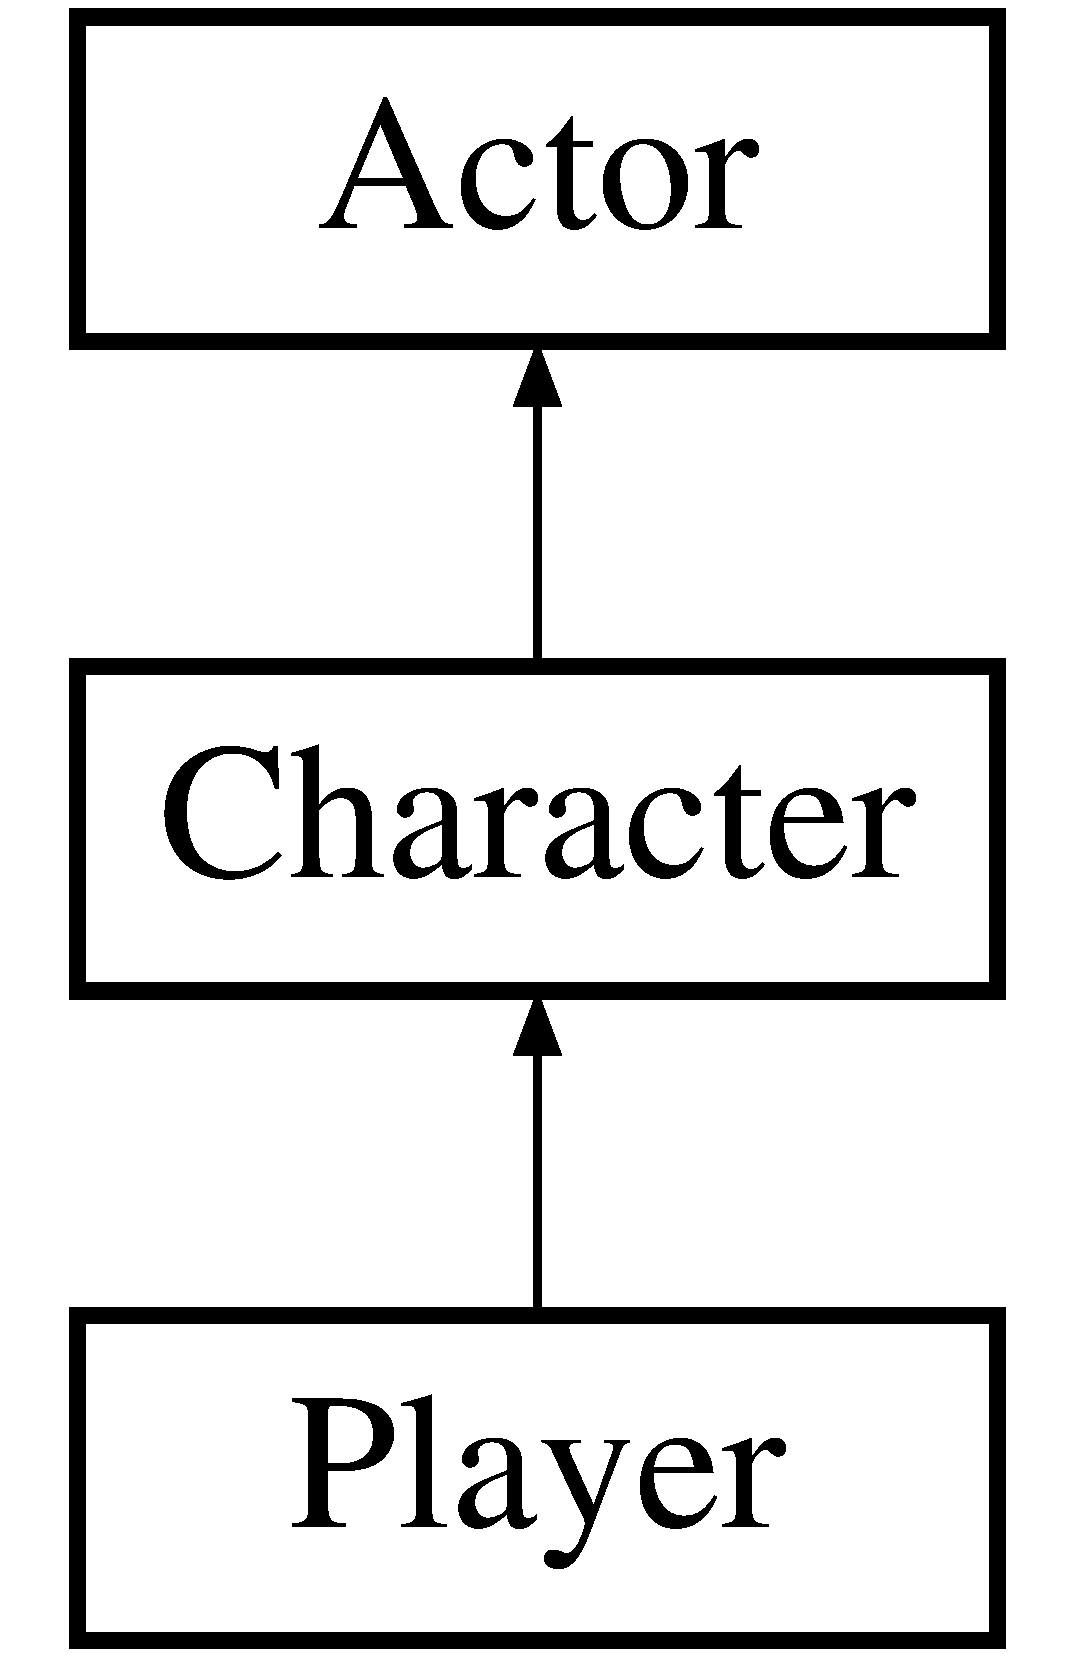
\includegraphics[height=3.000000cm]{class_player}
\end{center}
\end{figure}
\subsection*{Public Member Functions}
\begin{DoxyCompactItemize}
\item 
\hyperlink{class_player_affe0cc3cb714f6deb4e62f0c0d3f1fd8}{Player} ()
\item 
\hyperlink{class_player_af5aaea393030f959d568c806ca9100ca}{Player} (std\-::string name)
\end{DoxyCompactItemize}
\subsection*{Private Attributes}
\begin{DoxyCompactItemize}
\item 
short \hyperlink{class_player_a9ff033e2fbc16cd9eec507c0832cf1fa}{m\-\_\-sh\-Total\-Souls}
\item 
short \hyperlink{class_player_ac15acaec6575cc6ef5681aa3f8a23555}{m\-\_\-sh\-Current\-Souls}
\item 
short \hyperlink{class_player_aa4a137aee416bc314036eb2ec51e125a}{m\-\_\-sh\-Weapon\-Level}
\item 
short \hyperlink{class_player_aa495c787dc9c8f3861775efe6ab4c082}{m\-\_\-sh\-Armor\-Level}
\item 
std\-::string \hyperlink{class_player_a55507be1f64e7ba369b502b8fd3a12dd}{m\-\_\-s\-Name}
\end{DoxyCompactItemize}
\subsection*{Additional Inherited Members}


\subsection{Constructor \& Destructor Documentation}
\hypertarget{class_player_affe0cc3cb714f6deb4e62f0c0d3f1fd8}{\index{Player@{Player}!Player@{Player}}
\index{Player@{Player}!Player@{Player}}
\subsubsection[{Player}]{\setlength{\rightskip}{0pt plus 5cm}Player\-::\-Player (
\begin{DoxyParamCaption}
{}
\end{DoxyParamCaption}
)}}\label{class_player_affe0cc3cb714f6deb4e62f0c0d3f1fd8}
\hypertarget{class_player_af5aaea393030f959d568c806ca9100ca}{\index{Player@{Player}!Player@{Player}}
\index{Player@{Player}!Player@{Player}}
\subsubsection[{Player}]{\setlength{\rightskip}{0pt plus 5cm}Player\-::\-Player (
\begin{DoxyParamCaption}
\item[{std\-::string}]{name}
\end{DoxyParamCaption}
)}}\label{class_player_af5aaea393030f959d568c806ca9100ca}


\subsection{Member Data Documentation}
\hypertarget{class_player_aa495c787dc9c8f3861775efe6ab4c082}{\index{Player@{Player}!m\-\_\-sh\-Armor\-Level@{m\-\_\-sh\-Armor\-Level}}
\index{m\-\_\-sh\-Armor\-Level@{m\-\_\-sh\-Armor\-Level}!Player@{Player}}
\subsubsection[{m\-\_\-sh\-Armor\-Level}]{\setlength{\rightskip}{0pt plus 5cm}short Player\-::m\-\_\-sh\-Armor\-Level\hspace{0.3cm}{\ttfamily [private]}}}\label{class_player_aa495c787dc9c8f3861775efe6ab4c082}
\hypertarget{class_player_ac15acaec6575cc6ef5681aa3f8a23555}{\index{Player@{Player}!m\-\_\-sh\-Current\-Souls@{m\-\_\-sh\-Current\-Souls}}
\index{m\-\_\-sh\-Current\-Souls@{m\-\_\-sh\-Current\-Souls}!Player@{Player}}
\subsubsection[{m\-\_\-sh\-Current\-Souls}]{\setlength{\rightskip}{0pt plus 5cm}short Player\-::m\-\_\-sh\-Current\-Souls\hspace{0.3cm}{\ttfamily [private]}}}\label{class_player_ac15acaec6575cc6ef5681aa3f8a23555}
\hypertarget{class_player_a9ff033e2fbc16cd9eec507c0832cf1fa}{\index{Player@{Player}!m\-\_\-sh\-Total\-Souls@{m\-\_\-sh\-Total\-Souls}}
\index{m\-\_\-sh\-Total\-Souls@{m\-\_\-sh\-Total\-Souls}!Player@{Player}}
\subsubsection[{m\-\_\-sh\-Total\-Souls}]{\setlength{\rightskip}{0pt plus 5cm}short Player\-::m\-\_\-sh\-Total\-Souls\hspace{0.3cm}{\ttfamily [private]}}}\label{class_player_a9ff033e2fbc16cd9eec507c0832cf1fa}
\hypertarget{class_player_aa4a137aee416bc314036eb2ec51e125a}{\index{Player@{Player}!m\-\_\-sh\-Weapon\-Level@{m\-\_\-sh\-Weapon\-Level}}
\index{m\-\_\-sh\-Weapon\-Level@{m\-\_\-sh\-Weapon\-Level}!Player@{Player}}
\subsubsection[{m\-\_\-sh\-Weapon\-Level}]{\setlength{\rightskip}{0pt plus 5cm}short Player\-::m\-\_\-sh\-Weapon\-Level\hspace{0.3cm}{\ttfamily [private]}}}\label{class_player_aa4a137aee416bc314036eb2ec51e125a}
\hypertarget{class_player_a55507be1f64e7ba369b502b8fd3a12dd}{\index{Player@{Player}!m\-\_\-s\-Name@{m\-\_\-s\-Name}}
\index{m\-\_\-s\-Name@{m\-\_\-s\-Name}!Player@{Player}}
\subsubsection[{m\-\_\-s\-Name}]{\setlength{\rightskip}{0pt plus 5cm}std\-::string Player\-::m\-\_\-s\-Name\hspace{0.3cm}{\ttfamily [private]}}}\label{class_player_a55507be1f64e7ba369b502b8fd3a12dd}


The documentation for this class was generated from the following files\-:\begin{DoxyCompactItemize}
\item 
Game\-Project/\-Game\-Project/\hyperlink{_player_8h}{Player.\-h}\item 
Game\-Project/\-Game\-Project/\hyperlink{_player_8cpp}{Player.\-cpp}\end{DoxyCompactItemize}

\hypertarget{class_vector2f}{\section{Vector2f Class Reference}
\label{class_vector2f}\index{Vector2f@{Vector2f}}
}


{\ttfamily \#include $<$Vector2f.\-h$>$}

\subsection*{Public Member Functions}
\begin{DoxyCompactItemize}
\item 
\hyperlink{class_vector2f_a3db9a868c58bc809e5e09a88d65a77ec}{Vector2f} ()
\item 
\hyperlink{class_vector2f_ae3ff9026b0e1242471678e4f2ed8be0e}{Vector2f} (float \hyperlink{class_vector2f_add58d2378e3a3abdb76cf0ac51c9acfc}{x}, float \hyperlink{class_vector2f_a14874a72597fd358b15f8ba34b999c4d}{y})
\item 
\hyperlink{class_vector2f_a2f820078721656f1952f46b0861e19ef}{$\sim$\-Vector2f} ()
\item 
\hyperlink{class_vector2f}{Vector2f} \hyperlink{class_vector2f_acab3acffc23f8bf9ba36d61e06134e87}{operator+} (\hyperlink{class_vector2f}{Vector2f} vector)
\item 
\hyperlink{class_vector2f}{Vector2f} \hyperlink{class_vector2f_aabf72717e6da6001e9a3d01aeb9b2fc6}{operator-\/} (\hyperlink{class_vector2f}{Vector2f} vector)
\item 
\hyperlink{class_vector2f}{Vector2f} \hyperlink{class_vector2f_ab80cdeb3e397a1b721333efa7dc2b413}{operator$\ast$} (\hyperlink{class_vector2f}{Vector2f} vector)
\item 
\hyperlink{class_vector2f}{Vector2f} \hyperlink{class_vector2f_a5c633ed193d68fe42094e226b7ed4b2e}{operator/} (\hyperlink{class_vector2f}{Vector2f} vector)
\item 
void \hyperlink{class_vector2f_a5e7851b6e79d053d18d8330bd368043b}{operator=} (\hyperlink{class_vector2f}{Vector2f} vector)
\item 
\hyperlink{class_vector2f}{Vector2f} \hyperlink{class_vector2f_a580187e290048e034ec42c389e170f9e}{operator$\ast$} (float scalar)
\item 
\hyperlink{class_vector2f}{Vector2f} \hyperlink{class_vector2f_a1af75ea153e922fed0ea92bb68950157}{operator/} (float scalar)
\item 
float \hyperlink{class_vector2f_a28ef3af858da3c412cfb1522cff08a1f}{dot} (\hyperlink{class_vector2f}{Vector2f} vector)
\item 
float \hyperlink{class_vector2f_a0dc5b93838aa574e8aa00202ace11b9d}{cross} (\hyperlink{class_vector2f}{Vector2f} vector)
\item 
float \hyperlink{class_vector2f_a747f9f110283fd63d127b16521ee6fdc}{length} ()
\item 
\hyperlink{class_vector2f}{Vector2f} \hyperlink{class_vector2f_a6781e87d4d26cfc5d10a17e25c870f75}{unit} ()
\item 
float \hyperlink{class_vector2f_ac764933194f295f7671f36f32488ffb9}{squared\-Length} ()
\item 
\hyperlink{class_vector2f}{Vector2f} \hyperlink{class_vector2f_a877a04381f86f6157086c7901d460fc7}{turn\-Left} ()
\item 
\hyperlink{class_vector2f}{Vector2f} \hyperlink{class_vector2f_af63c77fc78259eb26ea05113254ee7e3}{turn\-Right} ()
\item 
\hyperlink{class_vector2f}{Vector2f} \hyperlink{class_vector2f_a4b32222b718c1e0e00317b1390fc555b}{rotate} (float \hyperlink{class_vector2f_a2d8be50dd28dc0ba8c1dcf1ecada2a23}{angle})
\item 
float \hyperlink{class_vector2f_a2d8be50dd28dc0ba8c1dcf1ecada2a23}{angle} ()
\end{DoxyCompactItemize}
\subsection*{Public Attributes}
\begin{DoxyCompactItemize}
\item 
float \hyperlink{class_vector2f_add58d2378e3a3abdb76cf0ac51c9acfc}{x}
\item 
float \hyperlink{class_vector2f_a14874a72597fd358b15f8ba34b999c4d}{y}
\end{DoxyCompactItemize}


\subsection{Constructor \& Destructor Documentation}
\hypertarget{class_vector2f_a3db9a868c58bc809e5e09a88d65a77ec}{\index{Vector2f@{Vector2f}!Vector2f@{Vector2f}}
\index{Vector2f@{Vector2f}!Vector2f@{Vector2f}}
\subsubsection[{Vector2f}]{\setlength{\rightskip}{0pt plus 5cm}Vector2f\-::\-Vector2f (
\begin{DoxyParamCaption}
{}
\end{DoxyParamCaption}
)}}\label{class_vector2f_a3db9a868c58bc809e5e09a88d65a77ec}
\hypertarget{class_vector2f_ae3ff9026b0e1242471678e4f2ed8be0e}{\index{Vector2f@{Vector2f}!Vector2f@{Vector2f}}
\index{Vector2f@{Vector2f}!Vector2f@{Vector2f}}
\subsubsection[{Vector2f}]{\setlength{\rightskip}{0pt plus 5cm}Vector2f\-::\-Vector2f (
\begin{DoxyParamCaption}
\item[{float}]{x, }
\item[{float}]{y}
\end{DoxyParamCaption}
)}}\label{class_vector2f_ae3ff9026b0e1242471678e4f2ed8be0e}
\hypertarget{class_vector2f_a2f820078721656f1952f46b0861e19ef}{\index{Vector2f@{Vector2f}!$\sim$\-Vector2f@{$\sim$\-Vector2f}}
\index{$\sim$\-Vector2f@{$\sim$\-Vector2f}!Vector2f@{Vector2f}}
\subsubsection[{$\sim$\-Vector2f}]{\setlength{\rightskip}{0pt plus 5cm}Vector2f\-::$\sim$\-Vector2f (
\begin{DoxyParamCaption}
{}
\end{DoxyParamCaption}
)}}\label{class_vector2f_a2f820078721656f1952f46b0861e19ef}


\subsection{Member Function Documentation}
\hypertarget{class_vector2f_a2d8be50dd28dc0ba8c1dcf1ecada2a23}{\index{Vector2f@{Vector2f}!angle@{angle}}
\index{angle@{angle}!Vector2f@{Vector2f}}
\subsubsection[{angle}]{\setlength{\rightskip}{0pt plus 5cm}float Vector2f\-::angle (
\begin{DoxyParamCaption}
{}
\end{DoxyParamCaption}
)}}\label{class_vector2f_a2d8be50dd28dc0ba8c1dcf1ecada2a23}
\hypertarget{class_vector2f_a0dc5b93838aa574e8aa00202ace11b9d}{\index{Vector2f@{Vector2f}!cross@{cross}}
\index{cross@{cross}!Vector2f@{Vector2f}}
\subsubsection[{cross}]{\setlength{\rightskip}{0pt plus 5cm}float Vector2f\-::cross (
\begin{DoxyParamCaption}
\item[{{\bf Vector2f}}]{vector}
\end{DoxyParamCaption}
)}}\label{class_vector2f_a0dc5b93838aa574e8aa00202ace11b9d}
\hypertarget{class_vector2f_a28ef3af858da3c412cfb1522cff08a1f}{\index{Vector2f@{Vector2f}!dot@{dot}}
\index{dot@{dot}!Vector2f@{Vector2f}}
\subsubsection[{dot}]{\setlength{\rightskip}{0pt plus 5cm}float Vector2f\-::dot (
\begin{DoxyParamCaption}
\item[{{\bf Vector2f}}]{vector}
\end{DoxyParamCaption}
)}}\label{class_vector2f_a28ef3af858da3c412cfb1522cff08a1f}
\hypertarget{class_vector2f_a747f9f110283fd63d127b16521ee6fdc}{\index{Vector2f@{Vector2f}!length@{length}}
\index{length@{length}!Vector2f@{Vector2f}}
\subsubsection[{length}]{\setlength{\rightskip}{0pt plus 5cm}float Vector2f\-::length (
\begin{DoxyParamCaption}
{}
\end{DoxyParamCaption}
)}}\label{class_vector2f_a747f9f110283fd63d127b16521ee6fdc}
\hypertarget{class_vector2f_ab80cdeb3e397a1b721333efa7dc2b413}{\index{Vector2f@{Vector2f}!operator$\ast$@{operator$\ast$}}
\index{operator$\ast$@{operator$\ast$}!Vector2f@{Vector2f}}
\subsubsection[{operator$\ast$}]{\setlength{\rightskip}{0pt plus 5cm}{\bf Vector2f} Vector2f\-::operator$\ast$ (
\begin{DoxyParamCaption}
\item[{{\bf Vector2f}}]{vector}
\end{DoxyParamCaption}
)}}\label{class_vector2f_ab80cdeb3e397a1b721333efa7dc2b413}
\hypertarget{class_vector2f_a580187e290048e034ec42c389e170f9e}{\index{Vector2f@{Vector2f}!operator$\ast$@{operator$\ast$}}
\index{operator$\ast$@{operator$\ast$}!Vector2f@{Vector2f}}
\subsubsection[{operator$\ast$}]{\setlength{\rightskip}{0pt plus 5cm}{\bf Vector2f} Vector2f\-::operator$\ast$ (
\begin{DoxyParamCaption}
\item[{float}]{scalar}
\end{DoxyParamCaption}
)}}\label{class_vector2f_a580187e290048e034ec42c389e170f9e}
\hypertarget{class_vector2f_acab3acffc23f8bf9ba36d61e06134e87}{\index{Vector2f@{Vector2f}!operator+@{operator+}}
\index{operator+@{operator+}!Vector2f@{Vector2f}}
\subsubsection[{operator+}]{\setlength{\rightskip}{0pt plus 5cm}{\bf Vector2f} Vector2f\-::operator+ (
\begin{DoxyParamCaption}
\item[{{\bf Vector2f}}]{vector}
\end{DoxyParamCaption}
)}}\label{class_vector2f_acab3acffc23f8bf9ba36d61e06134e87}
\hypertarget{class_vector2f_aabf72717e6da6001e9a3d01aeb9b2fc6}{\index{Vector2f@{Vector2f}!operator-\/@{operator-\/}}
\index{operator-\/@{operator-\/}!Vector2f@{Vector2f}}
\subsubsection[{operator-\/}]{\setlength{\rightskip}{0pt plus 5cm}{\bf Vector2f} Vector2f\-::operator-\/ (
\begin{DoxyParamCaption}
\item[{{\bf Vector2f}}]{vector}
\end{DoxyParamCaption}
)}}\label{class_vector2f_aabf72717e6da6001e9a3d01aeb9b2fc6}
\hypertarget{class_vector2f_a5c633ed193d68fe42094e226b7ed4b2e}{\index{Vector2f@{Vector2f}!operator/@{operator/}}
\index{operator/@{operator/}!Vector2f@{Vector2f}}
\subsubsection[{operator/}]{\setlength{\rightskip}{0pt plus 5cm}{\bf Vector2f} Vector2f\-::operator/ (
\begin{DoxyParamCaption}
\item[{{\bf Vector2f}}]{vector}
\end{DoxyParamCaption}
)}}\label{class_vector2f_a5c633ed193d68fe42094e226b7ed4b2e}
\hypertarget{class_vector2f_a1af75ea153e922fed0ea92bb68950157}{\index{Vector2f@{Vector2f}!operator/@{operator/}}
\index{operator/@{operator/}!Vector2f@{Vector2f}}
\subsubsection[{operator/}]{\setlength{\rightskip}{0pt plus 5cm}{\bf Vector2f} Vector2f\-::operator/ (
\begin{DoxyParamCaption}
\item[{float}]{scalar}
\end{DoxyParamCaption}
)}}\label{class_vector2f_a1af75ea153e922fed0ea92bb68950157}
\hypertarget{class_vector2f_a5e7851b6e79d053d18d8330bd368043b}{\index{Vector2f@{Vector2f}!operator=@{operator=}}
\index{operator=@{operator=}!Vector2f@{Vector2f}}
\subsubsection[{operator=}]{\setlength{\rightskip}{0pt plus 5cm}void Vector2f\-::operator= (
\begin{DoxyParamCaption}
\item[{{\bf Vector2f}}]{vector}
\end{DoxyParamCaption}
)}}\label{class_vector2f_a5e7851b6e79d053d18d8330bd368043b}
\hypertarget{class_vector2f_a4b32222b718c1e0e00317b1390fc555b}{\index{Vector2f@{Vector2f}!rotate@{rotate}}
\index{rotate@{rotate}!Vector2f@{Vector2f}}
\subsubsection[{rotate}]{\setlength{\rightskip}{0pt plus 5cm}{\bf Vector2f} Vector2f\-::rotate (
\begin{DoxyParamCaption}
\item[{float}]{angle}
\end{DoxyParamCaption}
)}}\label{class_vector2f_a4b32222b718c1e0e00317b1390fc555b}
\hypertarget{class_vector2f_ac764933194f295f7671f36f32488ffb9}{\index{Vector2f@{Vector2f}!squared\-Length@{squared\-Length}}
\index{squared\-Length@{squared\-Length}!Vector2f@{Vector2f}}
\subsubsection[{squared\-Length}]{\setlength{\rightskip}{0pt plus 5cm}float Vector2f\-::squared\-Length (
\begin{DoxyParamCaption}
{}
\end{DoxyParamCaption}
)}}\label{class_vector2f_ac764933194f295f7671f36f32488ffb9}
\hypertarget{class_vector2f_a877a04381f86f6157086c7901d460fc7}{\index{Vector2f@{Vector2f}!turn\-Left@{turn\-Left}}
\index{turn\-Left@{turn\-Left}!Vector2f@{Vector2f}}
\subsubsection[{turn\-Left}]{\setlength{\rightskip}{0pt plus 5cm}{\bf Vector2f} Vector2f\-::turn\-Left (
\begin{DoxyParamCaption}
{}
\end{DoxyParamCaption}
)}}\label{class_vector2f_a877a04381f86f6157086c7901d460fc7}
\hypertarget{class_vector2f_af63c77fc78259eb26ea05113254ee7e3}{\index{Vector2f@{Vector2f}!turn\-Right@{turn\-Right}}
\index{turn\-Right@{turn\-Right}!Vector2f@{Vector2f}}
\subsubsection[{turn\-Right}]{\setlength{\rightskip}{0pt plus 5cm}{\bf Vector2f} Vector2f\-::turn\-Right (
\begin{DoxyParamCaption}
{}
\end{DoxyParamCaption}
)}}\label{class_vector2f_af63c77fc78259eb26ea05113254ee7e3}
\hypertarget{class_vector2f_a6781e87d4d26cfc5d10a17e25c870f75}{\index{Vector2f@{Vector2f}!unit@{unit}}
\index{unit@{unit}!Vector2f@{Vector2f}}
\subsubsection[{unit}]{\setlength{\rightskip}{0pt plus 5cm}{\bf Vector2f} Vector2f\-::unit (
\begin{DoxyParamCaption}
{}
\end{DoxyParamCaption}
)}}\label{class_vector2f_a6781e87d4d26cfc5d10a17e25c870f75}


\subsection{Member Data Documentation}
\hypertarget{class_vector2f_add58d2378e3a3abdb76cf0ac51c9acfc}{\index{Vector2f@{Vector2f}!x@{x}}
\index{x@{x}!Vector2f@{Vector2f}}
\subsubsection[{x}]{\setlength{\rightskip}{0pt plus 5cm}float Vector2f\-::x}}\label{class_vector2f_add58d2378e3a3abdb76cf0ac51c9acfc}
\hypertarget{class_vector2f_a14874a72597fd358b15f8ba34b999c4d}{\index{Vector2f@{Vector2f}!y@{y}}
\index{y@{y}!Vector2f@{Vector2f}}
\subsubsection[{y}]{\setlength{\rightskip}{0pt plus 5cm}float Vector2f\-::y}}\label{class_vector2f_a14874a72597fd358b15f8ba34b999c4d}


The documentation for this class was generated from the following files\-:\begin{DoxyCompactItemize}
\item 
Game\-Project/\-Game\-Project/\hyperlink{_vector2f_8h}{Vector2f.\-h}\item 
Game\-Project/\-Game\-Project/\hyperlink{_vector2f_8cpp}{Vector2f.\-cpp}\end{DoxyCompactItemize}

\chapter{File Documentation}
\hypertarget{_actor_8cpp}{\section{Game\-Project/\-Game\-Project/\-Actor.cpp File Reference}
\label{_actor_8cpp}\index{Game\-Project/\-Game\-Project/\-Actor.\-cpp@{Game\-Project/\-Game\-Project/\-Actor.\-cpp}}
}
{\ttfamily \#include \char`\"{}Actor.\-h\char`\"{}}\\*

\hypertarget{_actor_8h}{\section{Game\-Project/\-Game\-Project/\-Actor.h File Reference}
\label{_actor_8h}\index{Game\-Project/\-Game\-Project/\-Actor.\-h@{Game\-Project/\-Game\-Project/\-Actor.\-h}}
}
{\ttfamily \#include \char`\"{}Vector2f.\-h\char`\"{}}\\*
{\ttfamily \#include \char`\"{}S\-F\-M\-L/\-Graphics.\-hpp\char`\"{}}\\*
\subsection*{Classes}
\begin{DoxyCompactItemize}
\item 
class \hyperlink{class_actor}{Actor}
\end{DoxyCompactItemize}

\hypertarget{_character_8cpp}{\section{Game\-Project/\-Game\-Project/\-Character.cpp File Reference}
\label{_character_8cpp}\index{Game\-Project/\-Game\-Project/\-Character.\-cpp@{Game\-Project/\-Game\-Project/\-Character.\-cpp}}
}
{\ttfamily \#include \char`\"{}Character.\-h\char`\"{}}\\*
\subsection*{Variables}
\begin{DoxyCompactItemize}
\item 
const short \hyperlink{_character_8cpp_a9235cdfc6201157b4738ee190b0e64e6}{B\-A\-S\-E\-\_\-\-S\-T\-A\-T} = 5
\end{DoxyCompactItemize}


\subsection{Variable Documentation}
\hypertarget{_character_8cpp_a9235cdfc6201157b4738ee190b0e64e6}{\index{Character.\-cpp@{Character.\-cpp}!B\-A\-S\-E\-\_\-\-S\-T\-A\-T@{B\-A\-S\-E\-\_\-\-S\-T\-A\-T}}
\index{B\-A\-S\-E\-\_\-\-S\-T\-A\-T@{B\-A\-S\-E\-\_\-\-S\-T\-A\-T}!Character.cpp@{Character.\-cpp}}
\subsubsection[{B\-A\-S\-E\-\_\-\-S\-T\-A\-T}]{\setlength{\rightskip}{0pt plus 5cm}const short B\-A\-S\-E\-\_\-\-S\-T\-A\-T = 5}}\label{_character_8cpp_a9235cdfc6201157b4738ee190b0e64e6}

\hypertarget{_character_8h}{\section{Game\-Project/\-Game\-Project/\-Character.h File Reference}
\label{_character_8h}\index{Game\-Project/\-Game\-Project/\-Character.\-h@{Game\-Project/\-Game\-Project/\-Character.\-h}}
}
{\ttfamily \#include \char`\"{}Actor.\-h\char`\"{}}\\*
\subsection*{Classes}
\begin{DoxyCompactItemize}
\item 
class \hyperlink{class_character}{Character}
\end{DoxyCompactItemize}

\hypertarget{_enemy_8h}{\section{Game\-Project/\-Game\-Project/\-Enemy.h File Reference}
\label{_enemy_8h}\index{Game\-Project/\-Game\-Project/\-Enemy.\-h@{Game\-Project/\-Game\-Project/\-Enemy.\-h}}
}

\hypertarget{_enemy_factory_8h}{\section{Game\-Project/\-Game\-Project/\-Enemy\-Factory.h File Reference}
\label{_enemy_factory_8h}\index{Game\-Project/\-Game\-Project/\-Enemy\-Factory.\-h@{Game\-Project/\-Game\-Project/\-Enemy\-Factory.\-h}}
}

\hypertarget{_enemy_handler_8h}{\section{Game\-Project/\-Game\-Project/\-Enemy\-Handler.h File Reference}
\label{_enemy_handler_8h}\index{Game\-Project/\-Game\-Project/\-Enemy\-Handler.\-h@{Game\-Project/\-Game\-Project/\-Enemy\-Handler.\-h}}
}

\hypertarget{_environment_8h}{\section{Game\-Project/\-Game\-Project/\-Environment.h File Reference}
\label{_environment_8h}\index{Game\-Project/\-Game\-Project/\-Environment.\-h@{Game\-Project/\-Game\-Project/\-Environment.\-h}}
}

\hypertarget{_game_8cpp}{\section{Game\-Project/\-Game\-Project/\-Game.cpp File Reference}
\label{_game_8cpp}\index{Game\-Project/\-Game\-Project/\-Game.\-cpp@{Game\-Project/\-Game\-Project/\-Game.\-cpp}}
}
{\ttfamily \#include \char`\"{}Game.\-h\char`\"{}}\\*

\hypertarget{_game_8h}{\section{Game\-Project/\-Game\-Project/\-Game.h File Reference}
\label{_game_8h}\index{Game\-Project/\-Game\-Project/\-Game.\-h@{Game\-Project/\-Game\-Project/\-Game.\-h}}
}
{\ttfamily \#include $<$S\-F\-M\-L/\-Graphics.\-hpp$>$}\\*
{\ttfamily \#include $<$S\-F\-M\-L/\-System/\-Clock.\-hpp$>$}\\*
{\ttfamily \#include $<$stdlib.\-h$>$}\\*
{\ttfamily \#include $<$iostream$>$}\\*
\subsection*{Classes}
\begin{DoxyCompactItemize}
\item 
class \hyperlink{class_game}{Game}
\end{DoxyCompactItemize}

\hypertarget{main_8cpp}{\section{Game\-Project/\-Game\-Project/main.cpp File Reference}
\label{main_8cpp}\index{Game\-Project/\-Game\-Project/main.\-cpp@{Game\-Project/\-Game\-Project/main.\-cpp}}
}
{\ttfamily \#include \char`\"{}Game.\-h\char`\"{}}\\*
\subsection*{Functions}
\begin{DoxyCompactItemize}
\item 
int \hyperlink{main_8cpp_ae66f6b31b5ad750f1fe042a706a4e3d4}{main} ()
\end{DoxyCompactItemize}


\subsection{Function Documentation}
\hypertarget{main_8cpp_ae66f6b31b5ad750f1fe042a706a4e3d4}{\index{main.\-cpp@{main.\-cpp}!main@{main}}
\index{main@{main}!main.cpp@{main.\-cpp}}
\subsubsection[{main}]{\setlength{\rightskip}{0pt plus 5cm}int main (
\begin{DoxyParamCaption}
{}
\end{DoxyParamCaption}
)}}\label{main_8cpp_ae66f6b31b5ad750f1fe042a706a4e3d4}

\hypertarget{_objects_8h}{\section{Game\-Project/\-Game\-Project/\-Objects.h File Reference}
\label{_objects_8h}\index{Game\-Project/\-Game\-Project/\-Objects.\-h@{Game\-Project/\-Game\-Project/\-Objects.\-h}}
}

\hypertarget{_player_8cpp}{\section{Game\-Project/\-Game\-Project/\-Player.cpp File Reference}
\label{_player_8cpp}\index{Game\-Project/\-Game\-Project/\-Player.\-cpp@{Game\-Project/\-Game\-Project/\-Player.\-cpp}}
}
{\ttfamily \#include \char`\"{}Player.\-h\char`\"{}}\\*

\hypertarget{_player_8h}{\section{Game\-Project/\-Game\-Project/\-Player.h File Reference}
\label{_player_8h}\index{Game\-Project/\-Game\-Project/\-Player.\-h@{Game\-Project/\-Game\-Project/\-Player.\-h}}
}
{\ttfamily \#include \char`\"{}Character.\-h\char`\"{}}\\*
\subsection*{Classes}
\begin{DoxyCompactItemize}
\item 
class \hyperlink{class_player}{Player}
\end{DoxyCompactItemize}

\hypertarget{_scene_handler_8h}{\section{Game\-Project/\-Game\-Project/\-Scene\-Handler.h File Reference}
\label{_scene_handler_8h}\index{Game\-Project/\-Game\-Project/\-Scene\-Handler.\-h@{Game\-Project/\-Game\-Project/\-Scene\-Handler.\-h}}
}

\hypertarget{_vector2f_8cpp}{\section{Game\-Project/\-Game\-Project/\-Vector2f.cpp File Reference}
\label{_vector2f_8cpp}\index{Game\-Project/\-Game\-Project/\-Vector2f.\-cpp@{Game\-Project/\-Game\-Project/\-Vector2f.\-cpp}}
}
{\ttfamily \#include \char`\"{}Vector2f.\-h\char`\"{}}\\*

\hypertarget{_vector2f_8h}{\section{Game\-Project/\-Game\-Project/\-Vector2f.h File Reference}
\label{_vector2f_8h}\index{Game\-Project/\-Game\-Project/\-Vector2f.\-h@{Game\-Project/\-Game\-Project/\-Vector2f.\-h}}
}
{\ttfamily \#include $<$math.\-h$>$}\\*
\subsection*{Classes}
\begin{DoxyCompactItemize}
\item 
class \hyperlink{class_vector2f}{Vector2f}
\end{DoxyCompactItemize}

\addcontentsline{toc}{part}{Index}
\printindex
\end{document}
